\section{Results}

\subsection{Verification of the geometry}\label{sec:mesh-verification}
The mesh and the mapping of section \ref{sec:dg-grid} are verified by integrating a smooth function over the sphere, for which the exact integral is known,
\begin{equation*}
    \int_S e^{\mathbf{a}\cdot\mathbf{n}}\,dA = 2\pi R^2\left(e - e^{-1}\right), \qquad |\mathbf{a}| = 1 .
\end{equation*}
This tests the vertices, the mapping, the Jacobian and the quadrature together. Figure \ref{fig:mesh-convergence} shows the relative error under $h$-refinement (increasing $n_I$) and $p$-refinement (increasing $N$). The total area of the elements also equals $4\pi R^2$ to within the quadrature error ($\approx 4\cdot10^{-7}$ relative for $n_I = 1$, $N = 4$, and below $10^{-8}$ for $n_I\geq2$), which confirms that the elements cover the sphere without gaps or overlaps.

\begin{figure}[H]
    \centering
    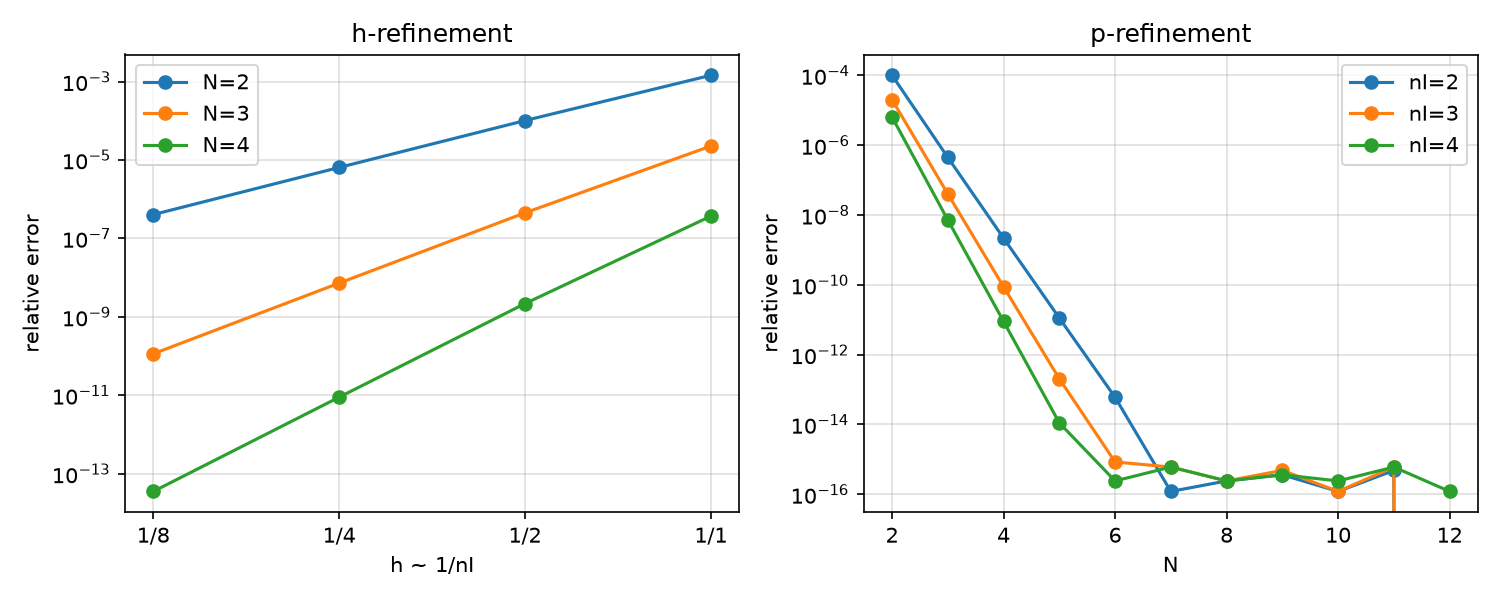
\includegraphics[width=0.9\textwidth]{Figures/convergence_integrals.png}
    \caption{Relative error of the integral of $e^{\mathbf{a}\cdot\mathbf{n}}$ over the sphere under $h$-refinement (left) and $p$-refinement (right).}
    \label{fig:mesh-convergence}
\end{figure}



\begin{figure}
    \centering
    \begin{subfigure}[t]{0.49\linewidth}
        \centering
        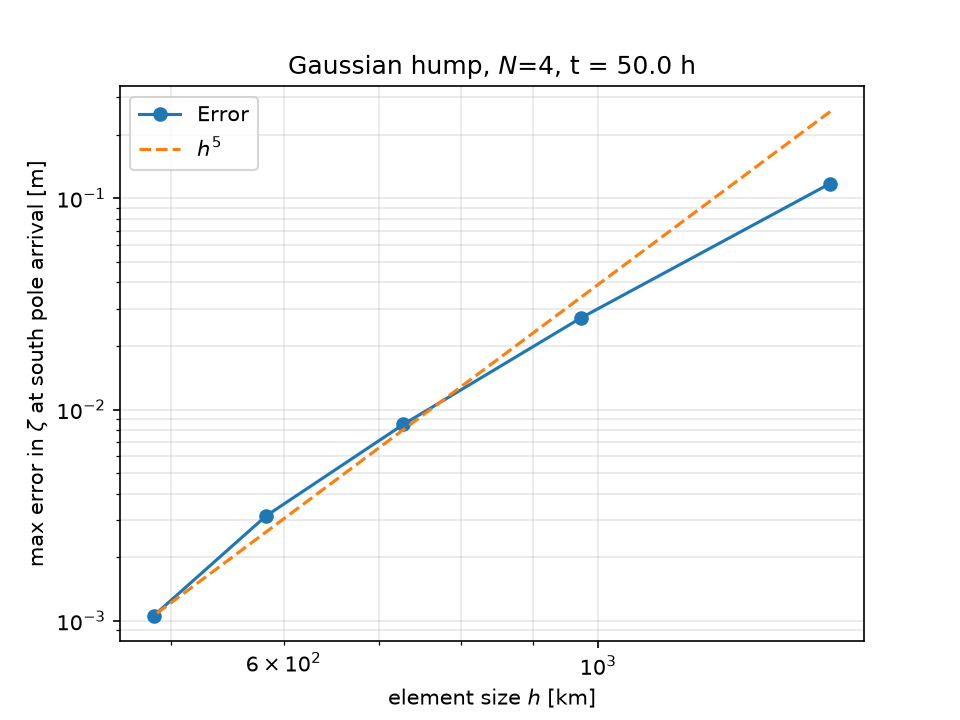
\includegraphics[width=\linewidth]{Figures/gaussian_hump_Hconvergence.png}
        \caption{h-convergence with $N=4$.}
        \label{fig:Hconvergence}
    \end{subfigure}
    \hfill
    \begin{subfigure}[t]{0.49\linewidth}
        \centering
        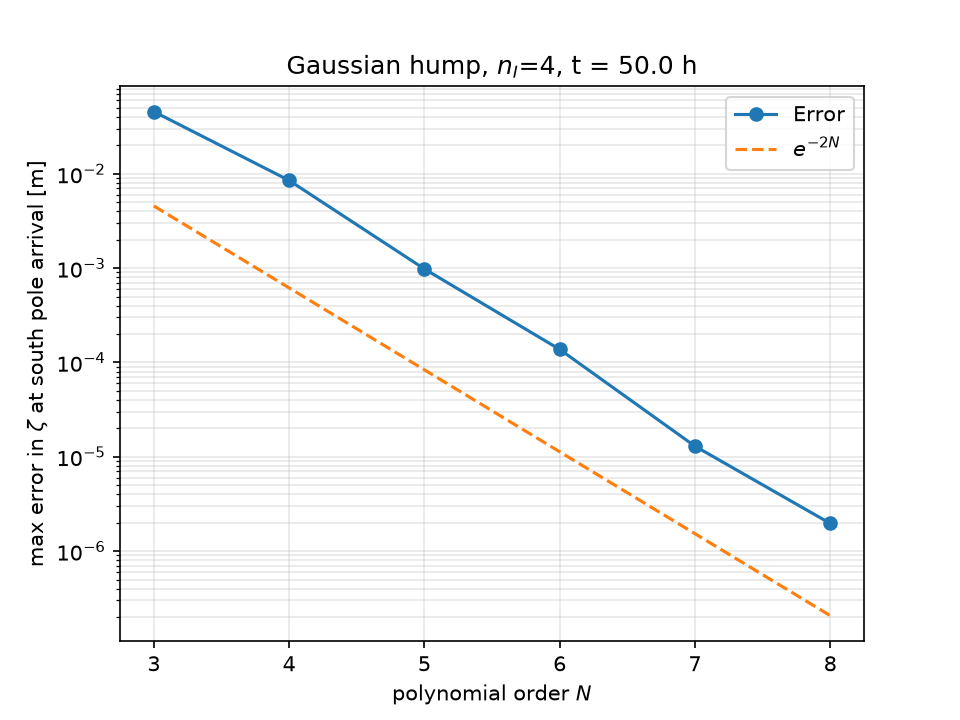
\includegraphics[width=\linewidth]{Figures/gaussian_hump_Pconvergence.png}
        \caption{p-convergence with $n_I=4$.}
        \label{fig:Pconvergence}
    \end{subfigure}
    \caption{Convergence for the Gaussian hump on the sphere. Linearized SWEs at time $t=50.0h$.}
    \label{fig:convergence}
\end{figure}

\begin{figure}
    \centering
    \begin{subfigure}[t]{0.32\linewidth}
        \centering
        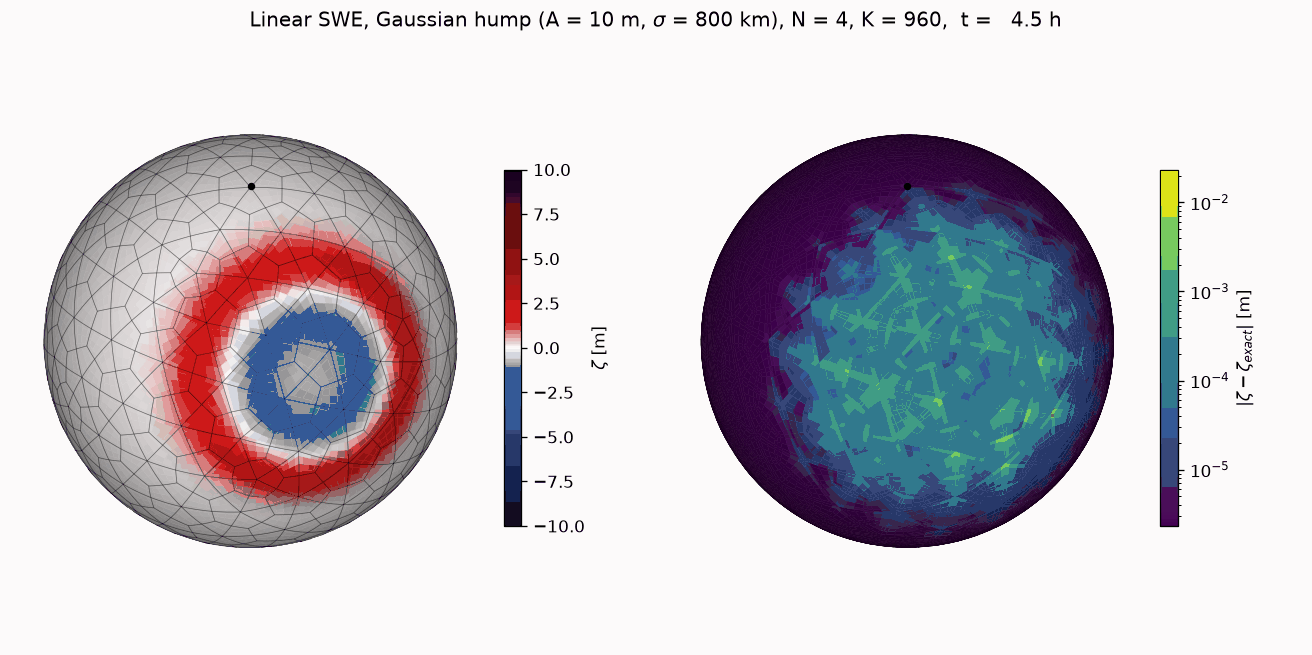
\includegraphics[width=\linewidth]{Figures/GIF_4-5h.png}
        \caption{Snapshot at 4.5h}
        \label{fig:snap4-5}
    \end{subfigure}
    \hfill
    \begin{subfigure}[t]{0.32\linewidth}
        \centering
        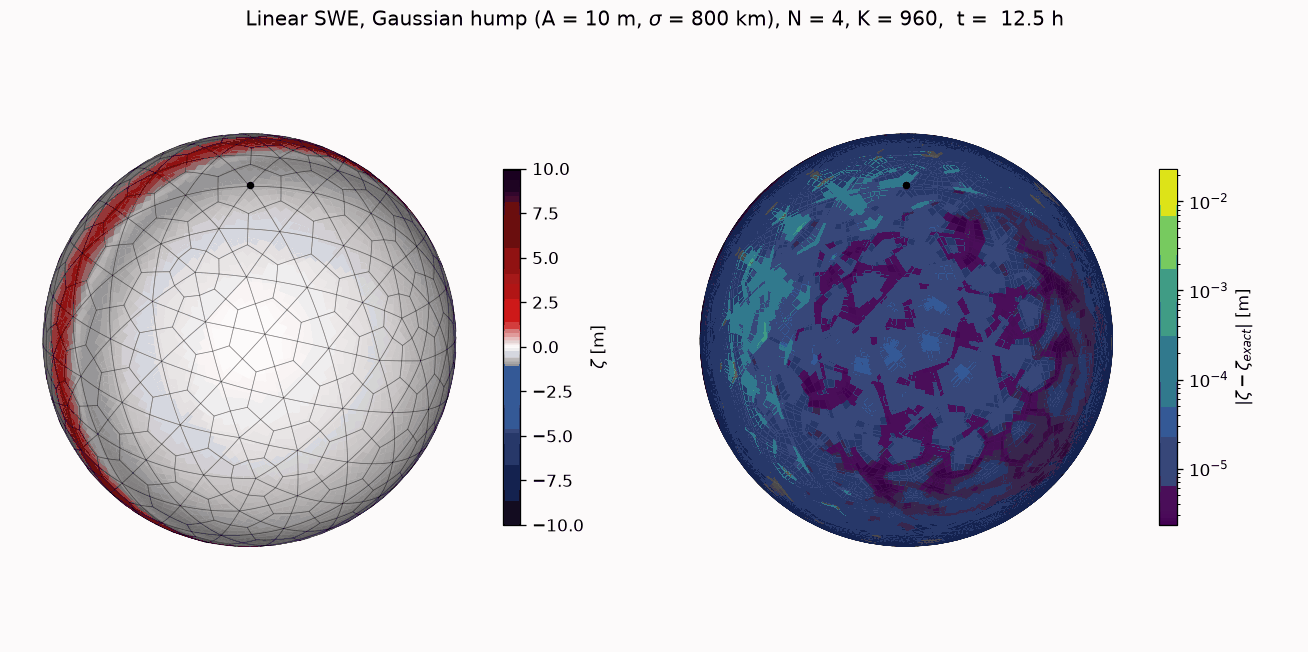
\includegraphics[width=\linewidth]{Figures/GIF_12-5h.png}
        \caption{Snapshot at 12.5h}
        \label{fig:snap12-5}
    \end{subfigure}
    \hfill
    \begin{subfigure}[t]{0.32\linewidth}
        \centering
        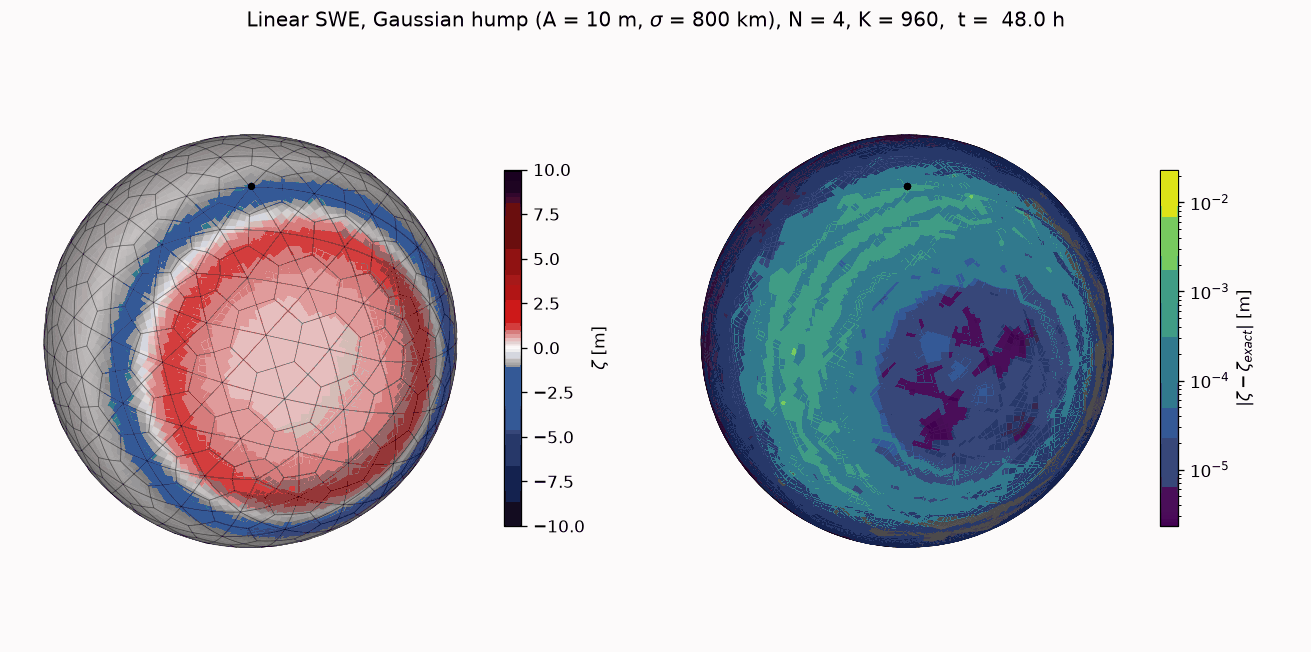
\includegraphics[width=\linewidth]{Figures/GIF_48h.png}
        \caption{Snapshot at 48h}
        \label{fig:snap48}
    \end{subfigure}
    \caption{Snapshots of animation of the wave travelling on the sphere}
    \label{fig:snapshots}
\end{figure}